\documentclass{article}

\usepackage[utf8]{inputenc}
\usepackage[dvipsnames]{xcolor}
\usepackage{lmodern}
\usepackage{graphicx}
\usepackage{longtable}
\usepackage{tabularx}
\graphicspath{ {../images/} }
\usepackage{imakeidx}
\makeindex[columns=3, title=Alphabetical Index, intoc]

\usepackage{tabularx}
\usepackage{amsmath}
\usepackage{paralist}
\usepackage{enumitem}
\usepackage{hyperref} %\usepackage[hidelinks]{hyperref} %per togliere bordi rossi
\usepackage{makecell}
\usepackage{caption}
\usepackage[maxfloats=256]{morefloats}
\maxdeadcycles=1000

\usepackage[official]{eurosym}
\DeclareUnicodeCharacter{20AC}{\euro{}}

\author{Agosta, Belli, Emili, Giacchini, Luciani}

\begin{document}

\begin{center}
    \sffamily{\fontsize{50}{48} \selectfont \textcolor{red}{Nexi}\textcolor{green}{Fy}}
\end{center}

\begin{center}
    \itshape{\fontsize{20}{48} \selectfont streaming to your pocket}
\end{center}

\bigskip\bigskip\bigskip

\begin{flushleft}
    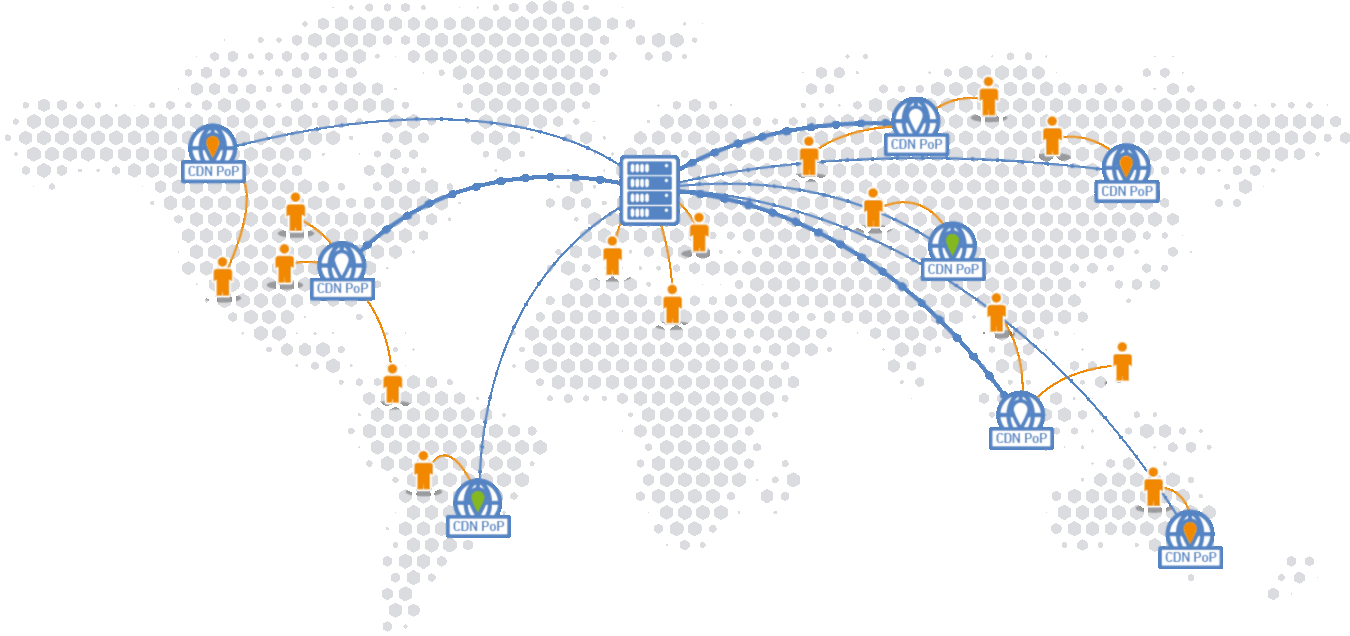
\includegraphics[scale=1]{../images/worldCDN.png}
\end{flushleft}

\bigskip\bigskip\bigskip

\begin{center}
    \itshape{\fontsize{30}{48} \selectfont Studio Di Fattibilit\'a}
\end{center}

\newpage
\printindex

\newpage
\section{\itshape{Studio di Fattibilità}}
\subsection{Aspetto tecnologico}
Per la realizzazione del sistema sarà necessario l'utilizzo di CDN, in modo da distribuire i contenuti multimediali in maniera efficiente e mantenendoli sempre accessibili per gli utenti. Deve inoltre essere possibile, in maniera efficiente, estrarre dati e statistiche dalla CDN (come per esempio quante volte è stato richiesto un certo video in una certa zona). Saranno necessarie basi di dati relazionali cloud-based per mantenere informazioni su dati utenti (oltre alle informazioni di base, anche le eventuali playlist musicali create, ecc), e implementando funzionalità lato server per gestire le richieste degli utenti, la loro autenticazione e altro. Verrà inoltre utilizzato un ORM per garantire semplicità di migrazione ad un'altra tecnologia di memorizzazione dati permettendo di rendere indipendente il codice dalla base di dati.\\
La fattibilità del progetto dal punto di vista tecnologico segue dalla grande disponibilità di aziende che offrono servizi cloud, tra cui CDN: per esempio AWS CloudFront. Questi servizi includono anche delle API per interfacciarsi in maniera efficiente con la CDN. Notiamo che questi servizi vengono già usati da piattaforme simili a NexiFy, e che sono risultate in grado di scalare a livello mondiale (ad esempio Prime Video usa AWS CloudFront). Anche per quanto riguarda i database esistono numerose soluzioni cloud affidabili.
%Il mantenimento dei dati riguardanti gli utenti sarà conforme alle politiche GDPR per garantire la privacy secondo le leggi europee.\\


%Per la realizzazione della piattaforma sarà necessario l’utilizzo di CDN per distribuire sul territorio contenuti multimediali mantenendo questi ultimi sempre accessibili in maniera ottimale da qualsiasi posizione geografica. Deve inoltre essere possibile, in maniera efficiente, estrarre dati e statistiche sugli accessi alla CDN. Si useranno basi di dati relazionali cloud-based per mantenere informazioni su dati utenti, e implementando funzionalità lato server per gestire le richieste degli utenti, la loro autenticazione e altro.Verrà inoltre utilizzato un ORM per garantire semplicità di migrazione ad un'altra tecnologia di memorizzazione dati permettendo di rendere indipendente il codice dalla base di dati.

\subsection{Aspetto Economico}
\subsubsection{Vantaggi del sistema}

NexiFy sarà in grado di acquisire utenti grazie ai diversi vantaggi offerti:
    \begin{itemize}
        \item La disponibilità di contenuti sia video che musicali, non presente in piattaforme quali Netflix e Spotify. Questo darà la possibilità agli utenti interessati di visualizzare film, serie tv e ascoltare brani musicali sottoscrivendo un singolo abbonamento, comportando un risparmio di denaro, in quanto non è necessario iscriversi a diversi servizi il cui costo totale ammonterebbe ad una quota mensile maggiore;
        \item La possibilità per piccoli creatori di pubblicare autonomamente contenuti, ma senza degradare la qualità dei contenuti (come invece avviene in piattaforme quali YouTube).

\subsubsection{Stima dei costi}
NexiFy inizialmente supporterà un numero modesto di utenti e di contenuti multimediali; questo per avere dei costi iniziali sostenibili, e man mano che si acquisiranno utenti (e quindi sottoscrizioni di abbonamenti) sarà possibile ampliare la CDN e i database (dal punto di vista software NexiFy sarà già progettato per supportare un carico maggiore del carico iniziale).

\textbf{todo... conti precisi}

    \end{itemize}
\index{Index}

\end{document}
